% Created for RoboCup Humanoid League by Professor Azer Babaev

\documentclass[a4paper]{article}
\usepackage{calc,amsmath,amssymb,amsfonts}
\usepackage[LGR,T1]{fontenc}
\usepackage{fouriernc}
\usepackage[greek,english]{babel}
\usepackage{xcolor,enumitem,hyperref}
\hypersetup{colorlinks=true,allcolors=blue}
\usepackage[pdftex]{graphicx}
% Pages
\renewcommand\thepage{\arabic{page}}
\newtheorem{theorem}{Theorem}
\begin{document}
%\large
\normalsize
{\centering
RoboCup Federation
\par}


\bigskip


\bigskip

{\centering
Humanoid League Major / Junior Bridging event
\par}


\bigskip

{\centering
(Humanoid Entry Level Soccer Initiative -HELSI)
\par}


\bigskip


\bigskip

{\centering
Rules and Setup
\par}

{\centering
for the 2025 competitions
\par}

{\centering
(Project)
\par}


\bigskip


\bigskip


\bigskip


\bigskip


\bigskip


\bigskip

{\centering
November 21st, 2024
\par}

{\centering
Compiled by Prof. Azer Babaev
\par}

{\centering
(Based on the 2007 version of the rules Humanoid Soccer)
\par}

{\centering
Dubai
\par}


\bigskip


\bigskip


\bigskip


\bigskip


\bigskip


\bigskip


\bigskip
\newpage

{\centering
\textbf{Abstract}
\par}

Current rules are designed for Humanoid League Junior and Major bridging event with abbreviation HELSI (Humanoid Entry
Level Soccer Initiative). \ Ages of students participating in teams are limited from experienced high school students
of last 2 forms and ungraduated (1-2 year) university-college students. Student team members are not allowed to
participate in world competitions more than 2 years. Games will be held on special carpet. The ball specified to be
orange coloured sponge tennis ball. Robot must be humanoid with number of D.O.F {\textless}= 25, weight {\textless} 3.3
kg, height {\textless} 60cm, with number of cameras {\textless}=2. It is preferred that team members have their
contribution into structure of robot. If robot is built by non-team members, then team members must perform their
individual contribution into algorithms in team poster and in TDP. Within tournament teams have to complete 5
challenges and participate in soccer game competition. Team can be admitted to soccer games in case of successful
completing at least one of challenges. Result of challenges will be solution of tie if two teams accumulate equal
number of points in soccer game competition. 


\bigskip

\textbf{\textcolor{black}{Table of Content}}

\textcolor{black}{\ \newline
1 The Field of
Play.................................................................................................\ \ 3\newline
2 The
Ball...............................................................................................................\ \ 4\newline
3 The Number of Players
......................................................................................\ \ 4\newline
4 The Design of the
Robots...................................................................................\ \ 5\newline
5 The Referee
.......................................................................................................\ \ 7\newline
6 The Assistant
Referees.......................................................................................\ \ 8\newline
7 The Duration of the
Match..................................................................................\ \ 8\newline
8 The Start and Restart of
Play.............................................................................\ \ 8\newline
9 The Ball In and Out of Play
................................................................................\ \ 9\newline
10 The Method of Scoring
.....................................................................................\ \ 9\newline
11
Offside..............................................................................................................\ \ 10\newline
12 Fouls and Misconduct
......................................................................................\ \ 10\newline
13 The Free Kicks
.................................................................................................\ \ 10\newline
14 The Penalty
Kick...............................................................................................\ \ 10\newline
15 The Throw-In
....................................................................................................\ \ 11\newline
16 The Goal
Kick...................................................................................................\ \ 11\newline
17 The Corner
Kick................................................................................................\ \ 11\newline
18 The
Footrace....................................................................................................\ \ 11\newline
19 The Technical
Challenge.................................................................................\ \ 11\newline
20 The Competitions and Trophies.......................................................................\ \ 14}


\bigskip


\bigskip
\newpage

\textbf{\textcolor{black}{1 The Field of Play}}

\textcolor{black}{\ The competitions take place on a rectangular field, which contains two goals, field lines, six
restart markers, as shown in Fig. 1.}

\textcolor{black}{Figure 1: Soccer field.}
\newline
 
%\begin{figure}
{\centering
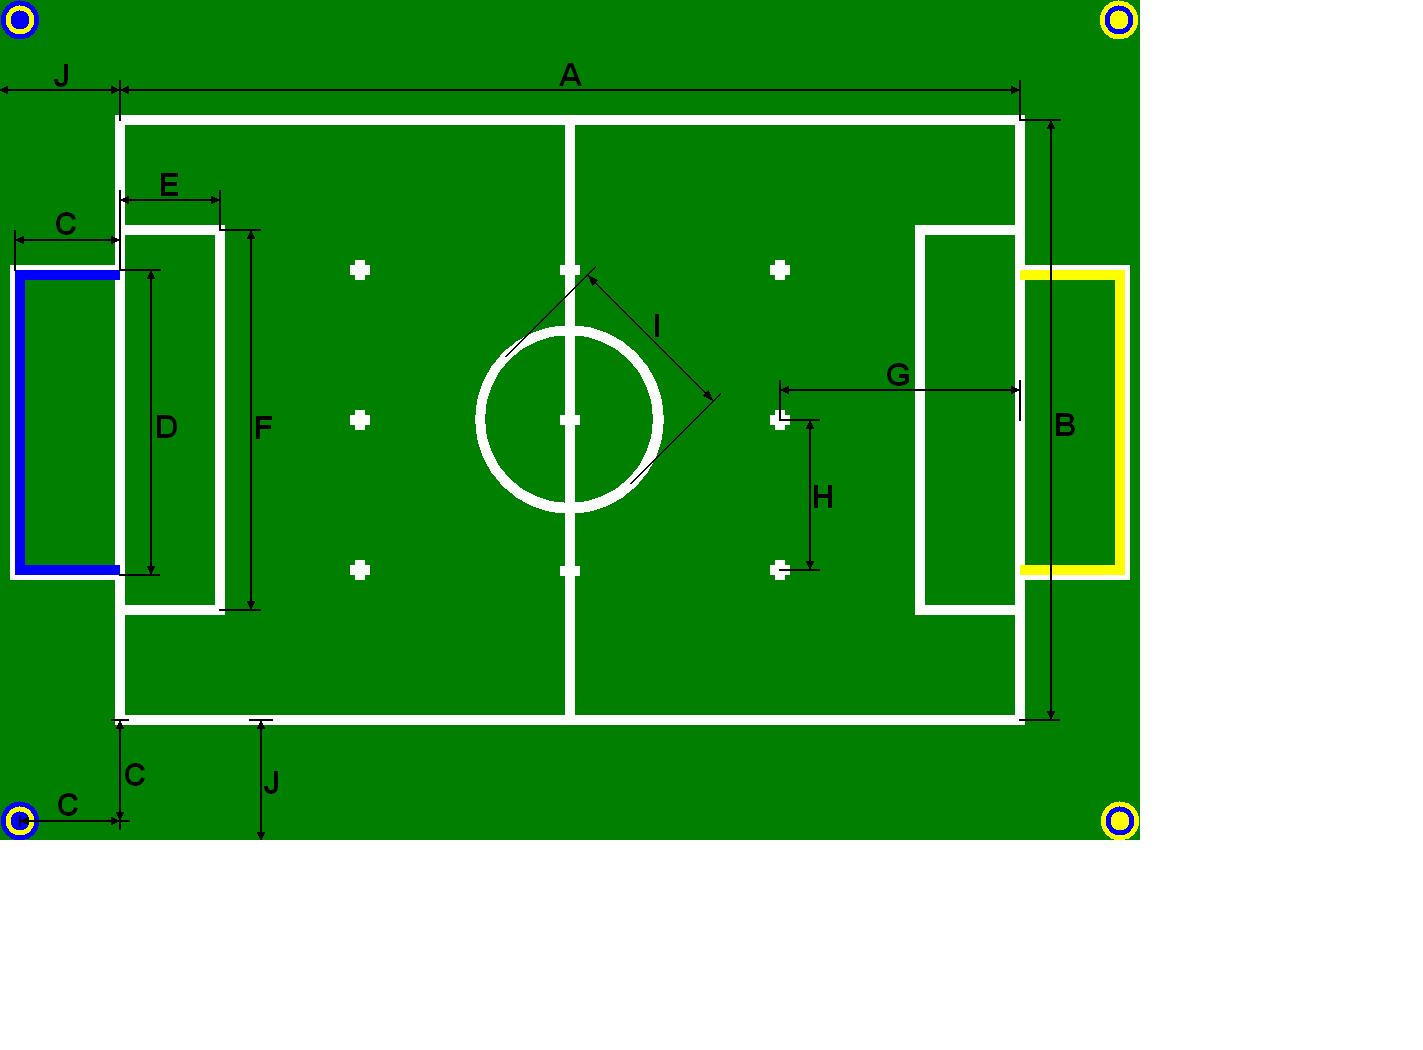
\includegraphics[width=16.058cm,height=11.85cm]{img/HELSI_rules_2025-img001.jpg}
}
%\end{figure}
\textcolor{black}{Table 1: Soccer field sizes, in cm.}\newline
\textbf{\textcolor{black}{ A }}\textcolor{black}{Field length \ \ \ \ }\textbf{\textcolor{black}{360}}\newline
\textbf{\textcolor{black}{ B }}\textcolor{black}{Field width \ \ \ \ }\textbf{\textcolor{black}{260}}\newline
\textbf{\textcolor{black}{ C }}\textcolor{black}{Goal length \ \ }\textbf{\textcolor{black}{15}}\newline
\textbf{\textcolor{black}{ D }}\textcolor{black}{Goal width \ \ \ \ }\textbf{\textcolor{black}{100\newline
 E }}\textcolor{black}{Goal area length \ \ }\textbf{\textcolor{black}{20}}\newline
\textbf{\textcolor{black}{ F }}\textcolor{black}{Goal area width \ \ }\textbf{\textcolor{black}{140\newline
G }}\textcolor{black}{Penalty kick distance \ \ }\textbf{\textcolor{black}{90\newline
H }}\textcolor{black}{Restart marker width \ \ }\textbf{\textcolor{black}{65}}\newline
\textbf{\textcolor{black}{ I }}\textcolor{black}{Center circle diameter \ \ }\textbf{\textcolor{black}{60}}\newline
\textbf{\textcolor{black}{ J }}\textcolor{black}{Border strip width (min.) \ \ }\textbf{\textcolor{black}{20}}


\bigskip


\bigskip


\bigskip
\newpage

%\begin{enumerate}[series=listWWNumi,label=\arabic*]
%\item \begin{enumerate}[series=listWWNumi,label=\arabic{enumi}.\arabic*]
%\item {\color{black}
\textbf{1.1 Playing Surface}
%\end{enumerate}
%\end{enumerate}
\textcolor{black}{The field is covered with green carpet of 3mm thickness flat surface and flat bottom. }

\textcolor{black}{The white lines are 5cm wide. Line segments of 10cm length are used to mark penalty positions, restart
positions, and the kick-off position. The longer outer field lines are called touch lines, whereas the shorter outer
field lines are called}\textcolor{black}{ }\textcolor{red}{\ \ \ }\textcolor{black}{goal lines. The six restart
positions are located half-way between the axis connecting the two goals and the touch lines, three on each side: in
the middle and between the penalty positions and the touch lines. The field is surrounded by a border strip, which is
also covered with green carpet. The world outside the border strip is undefined.}

\textbf{\textcolor{black}{1.2 Goals}}

\textcolor{black}{A goal is placed in the middle of each goal line. One of the goals is colored yellow at the three
inner walls. The other goal is colored blue. The goals have a horizontal goal bar at a height of 60cm. The outer goal
walls, as well as the goal posts and the goal bar are colored white.}

\textbf{\textcolor{black}{1.3 People area}}

\textcolor{black}{\ Around the field of play (Figure 1) a field zone is defined on site in which only the referee
(Section 5), the assistant referees (Section 6) and the two robot handlers are allowed to stay during a game. All other
people (including other team members, organizational staff, representatives of the press and the media etc.) must stay
outside the field zone. Width of referee/handler\textgreek{’}s area is 1.5 meter.}

\textbf{\textcolor{black}{2 The Ball}}

\textcolor{black}{Orange foam sponge ball for tennis (8 cm diameter, 26g).}

\textbf{\textcolor{black}{3 The Number of Players}}

\textcolor{black}{\ A match is played by two teams, each consisting of not more than two players, one of whom may be
designated as goalkeeper. A match may not start if either team consists of less than one player.}


\bigskip

\textbf{\textcolor{black}{3.1 Incapable players}}

\textcolor{black}{\ Players not capable of play (e.g., players not walking on two legs, players not able to stand) are
not permitted to participate in the game. They must be removed from the field. It is up to the referee to judge whether
a player is incapable of play. A field player that is not able to get back into a standing or walking posture from a
fall within 20 seconds receives a 30 seconds removal penalty. If the ball is within a radius of 0.3 m around the goal
keeper inside the goal area, the goal keeper has to show active attempts to move the ball out of this radius by walking
towards the ball or moving the ball. If no attempt is shown for 20 seconds, the goal keeper is considered to be an
inactive player and receives a 30 seconds removal penalty.}

\textcolor{black}{A player that stays outside of the field for 20 seconds is considered as an incapable player and
receives a 30 seconds removal penalty.}


\bigskip

\textbf{\textcolor{black}{Removal Penalty.}}

\textcolor{black}{\ Time penalties of 30 seconds for players are called by the referee. A field player or goal keeper
suffering a time penalty will be automatically removed from the field by handler and is only allowed to re-enter the
field from the team's own half of the field close to the penalty mark as indicated by the referee. The referee chooses
the touch line further away from the ball if there is still an empty spot available. The first spot for a penalized
robot on the touch line is on the same height of the penalty mark. A valid position must be at least 30 cm away from
the goal line and center line. The referee always positions the robot on the penalty spot closest to the penalty mark.
If two positions are available that are equally close, the referee chooses the position that is further away from the
ball. After the robot has been placed at the position indicated by the referee and with both feet entirely outside the
field of play the 30 seconds penalty start counting.}


\bigskip

\textbf{3.2 Substitutions}

Up to two players per game can be substituted by other players of the same team. The referee must be informed prior to
the substitution. A substitute only enters the field after the player being replaced left the field and after receiving
a signal from the referee. Any of the other players may change places with the goalkeeper, provided that the referee is
informed before the change is made and that the change is made during a stoppage of the match. Exchanging a field
player with a goalie does not count as substitution.

\textbf{3.3 Temporal Absence}

\ Servicing robots on the playing field is not permitted. A robot may be taken out of the field for service, after
receiving permission from the referee. Taking out a robot for service does not count as a substitution. A serviced
robot may not come into play again before 30 seconds elapsed after it was taken out. It has to enter the field at the
position of a touch line closest to the position where it was taken out. It has to face the center of the field when
entering.

\textbf{4 The Design of the Robots}

Robots participating in the Humanoid League competitions must have a human-like body plan, as shown in Fig. 2. They must
consist of two legs, two arms, and one head, which are attached to a trunk. The robots must be able to stand upright on
their feet and to walk on their legs. The only allowed modes of locomotion are bipedal walking and running.

\textcolor{black}{Figure 2: Humanoid robot body plan.}

%\begin{figure}
{\centering
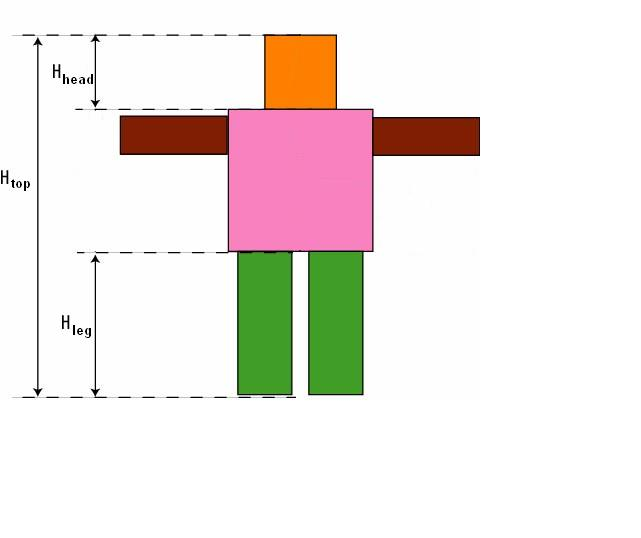
\includegraphics[width=7.234cm,height=6.07cm]{img/HELSI_rules_2025-img002.jpg}}
%\end{figure}
\textbf{\textcolor{black}{4.1 Robot Height}}

\textbf{\textcolor{black}{4.1.1: }}\textcolor{black}{The height H of a robot is determined as follows:}

\textcolor{black}{H = min(Htop, 2.2 \textgreek{· }H}\textcolor{black}{\textsubscript{com}}\textcolor{black}{),}

\textcolor{black}{\ where H}\textcolor{black}{\textsubscript{top }}\textcolor{black}{denotes the height of the robot
when standing upright and H}\textcolor{black}{\textsubscript{com }}\textcolor{black}{denotes the height of the robot's
center of mass, measured in upright posture.}


\bigskip

\textbf{\textcolor{black}{4.2 Size Restrictions}}

\textcolor{black}{All robots participating in the Humanoid League must comply with the following restrictions:}

\textcolor{black}{4.2.1. Each foot must fit into a rectangle of area
H}\textcolor{black}{\textsuperscript{2}}\textcolor{black}{/24.}

\textcolor{black}{4.2.2. Considering the rectangle enclosing the convex hull of the foot, the ratio between the longest
side of the rectangle and the shortest one, shall not exceed 2.5\newline
 4.2.3. The robot must fit into a cylinder of diameter 0.55*H.}

\textcolor{black}{4.2.4. If the arms are maximally stretched in horizontal direction, their extension must be less than
1.2 \textgreek{· }H.}

\textcolor{black}{4.2.5. The robot does not possess a configuration where it is extended longer than 1.5 \textgreek{·
}H.}

\textcolor{black}{4.2.6. The length of the legs H}\textcolor{black}{\textsubscript{leg}}\textcolor{black}{, including
the feet, satisfies 0.35\textgreek{·}H ${\leq}$ H}\textcolor{black}{\textsubscript{leg }}\textcolor{black}{${\leq}$
0.7\textgreek{·}H.\newline
 4.2.7. The height of the head H}\textcolor{black}{\textsubscript{head}}\textcolor{black}{, including the neck,
satisfies 0.05\textgreek{·}H ${\leq}$ H}\textcolor{black}{\textsubscript{head }}\textcolor{black}{${\leq}$
0.25\textgreek{·}H.}

\textcolor{black}{4.2.8. \ \ Weight of robot must be less than 3.3 kg. }

\textcolor{black}{4.2.9. \ 30 cm ${\leq}$ H ${\leq}$ 60 cm.}

\textbf{\textcolor{black}{4.3 Sensors}}

\textcolor{black}{Teams participating in the Humanoid League competitions are encouraged to equip their robots with
sensors that have an equivalent in humans. These sensors should be placed at a position roughly equivalent to the human
senses. In particular,}

\textcolor{black}{4.3.1. Any active sensor (emitting light, sound, or electromagnetic waves into the environment in
order to measure reflections) is not allowed.}

\textcolor{black}{4.3.2. External sensors, such as cameras and microphones, may not be placed in the legs or arms of the
robots. They should be placed in the robot's head.}

\textcolor{black}{4.3.3. Touch sensors, force sensors, and temperature sensors may be placed at any position on the
robot.}

\textcolor{black}{4.3.4. Sensors inside the robot may measure all quantities of interest, including (but not limited to)
voltages, currents, forces, movements, accelerations, and rotational speeds. Such sensors can be installed at any
position inside the robot.}


\bigskip

\textbf{\textcolor{black}{4.4 Communication and Control}}


\bigskip

\textcolor{black}{4.4.1: Robots participating in the competitions must act autonomously while a competition is running.
No external power supply, teleoperation, remote control, or remote brain of any kind is allowed.}

\textcolor{black}{4.4.2: Robots may communicate only via the wireless network. The robots must not rely on availability
or quality of the wireless network. They must be able to play if the network is not available or of low quality.}

\textcolor{black}{4.4.3: Robots of a team may communicate with each other at any time during a game. Communication to
external computer is not allowed during game.}

\textcolor{black}{4.4.4: No humans are allowed on the field while the ball is in play. Robot handlers must receive
permission from the referee prior to entering the field. Each team may designate }\textcolor{black}{only one person as
robot handler. The robot handler of a team may not touch a robot of another team in order to avoid any (unintentional
or intentional) damage to that robot.}

\textcolor{black}{4.4.5. Handler is allowed to activate robot to game by pressing button.}

\textcolor{black}{4.4.6. Each robot must be equipped with emergency STOP button which deactivates servomotors of robot.}


\bigskip

\textbf{\textcolor{black}{4.5 Colors and Markers}}

\textcolor{black}{4.5.1. Robots must be mostly black. Less than 10\% of the total body surface may have a higher
reflectance, e.g., gray or white. Less than 1\% of the total body surface may be colored. Any color used for the field
(green, yellow, blue) or the ball (orange) should be avoided.}

\textcolor{black}{4.5.2. The robots must be marked with team markers, attached to the trunk. These markers are colored
magenta for one team and cyan for the other team. Color marker of team must be at least 50 sq.cm at each robot. If both
teams cannot agree, which team color to use, a coin will be flipped 15 minutes prior to the game to assign the team
colors.}

\textcolor{black}{4.5.3. The robots of a team must be uniquely identifiable. They should be marked with numbers or
names.}


\bigskip

\textbf{\textcolor{black}{4.6 Robustness}}

\textcolor{black}{Robots participating in the Humanoid League competitions must be constructed in a robust way. They
must maintain structural integrity during contact with the field, the ball, or other players. Their sensing systems
must be able to tolerate significant levels of noise and disturbance caused by other players, the referees, robot
handlers, and the audience.}


\bigskip

\textbf{\textcolor{black}{5 The Referee}}

\textcolor{black}{5.1. Each match is controlled by a referee who has full authority to enforce these rules in connection
with the match to which he has been appointed.}

\textcolor{black}{5.2. The Referee ensures that the field and the ball are in proper condition. He ensures that the
robot players meet the requirements of Section 4.}

\textcolor{black}{5.3. The referee acts as timekeeper and keeps a record of the match. He stops, suspends or terminates
the match, at his discretion, for any infringements of the rules or because of outside interference of any kind.}

\textcolor{black}{5.4. The referee allows play to continue when the team against which an offense has been committed
will benefit from such an advantage and penalizes the original offense if the anticipated advantage does not ensue at
that time.}

\textcolor{black}{5.5. He punishes the more serious offense when a player commits more than one offense at the same time
and takes disciplinary action against players guilty of cautionable and sending-off offenses. He is not obliged to take
this action immediately but must do so when the ball next goes out of play.}

\textcolor{black}{5.6. The referee takes action against team officials who fail to conduct themselves in a responsible
manner and may, at his discretion, expel them from the field of play and its immediate surrounds. He ensures that no
unauthorized persons enter the field of play.}

\textcolor{black}{5.7. The referee acts on the advice of assistant referees regarding incidents which he has not seen.
Some referee duties, like time keeping and keeping a record of the match, may be delegated to one of the assistant
referees.}

\textcolor{black}{5.8. The decisions of the referee regarding facts connected with play are final. The referee may only
change a decision on realizing that it is incorrect or, at his discretion, on the advice of an assistant referee,
provided that he has not restarted play.}


\bigskip


\bigskip

\textbf{\textcolor{black}{6 The Assistant Referees}}

\textcolor{black}{6.1. One or more assistant referees are appointed for a match whose duties, subject to the decision of
the referee, are to indicate when the whole of the ball has passed out of the field of play, which side is entitled to
a corner kick, goal kick or throw-in, and when misconduct or any other incident has occurred out of the view of the
referee.}

\textcolor{black}{6.2. The assistant referees might be assigned additional duties, such as time keeping and keeping a
record of the match.}

\textcolor{black}{6.3. The assistant referees also assist the referee to control the match in accordance with these
rules.}

\textcolor{black}{6.4. In the event of undue interference or improper conduct, the referee will relieve an assistant
referee of his duties and make a report to the league organizing committee.}


\bigskip

\textbf{\textcolor{black}{7 The Duration of the Match}}

\textbf{\textcolor{black}{7.1 Periods}}

\textcolor{black}{7.1.1. The match lasts two equal periods of 5 minutes. Players are entitled to an interval at
half-time. The half-time interval must not exceed 5 minutes.}

\textcolor{black}{7.1.2. Allowance is made in either period for all time lost through, e.g., substitution(s), timeouts,
and wasting time. The allowance for time lost is at the discretion of the referee.}

\textcolor{black}{7.1.3. In the knock-out games of a tournament two further equal periods of 5 minutes each are played
if the game is not decided after the regular playing time. If during regular playing time none of the two teams in a
knock-out match was able to kick the ball to reach their respective opponent's goal the extra time is skipped and the
game immediately continues by the five alternating penalty kick trials (cf. Section 14).}

\textbf{\textcolor{black}{7.2 Timeouts}}

\textcolor{black}{\ A team may extend a stoppage of the game by taking a timeout. During a timeout robots may be
serviced. Each team may take at most one timeout per period. If a team is not ready to resume the game when the referee
wants to start the game, it has to take a timeout. If there is no timeout left, the referee will start the game anyway.
A timeout ends automatically after 120s. A timeout also ends when the team signals its end to the referee.}


\bigskip

\textbf{\textcolor{black}{8 The Start and Restart of Play}}

\textbf{\textcolor{black}{8.1 Preliminaries}}

\textcolor{black}{8.1.1. Access to the field is given to both teams at least 15 minutes prior to the scheduled kick-off
time. A coin is tossed and the team which wins the toss decides which goal it will attack in the first half of the
match. The other team takes the kick-off to start the match. The team which wins the toss takes the kick-off to start
the second half of the match. In the second half of the match the teams change ends and attack the opposite goals.}

\textcolor{black}{8.1.2. If both teams cannot agree on the color of their team makers, a coin is tossed and the markers
are exchanged at halftime.}

\textcolor{black}{8.1.3. A match must start at the scheduled time. In exceptional situations only, the referee may
re-adjust the time for starting the game in accordance with both team leaders. \ All robots of a team are started (and
stopped) manually by handlers.}

\textbf{\textcolor{black}{8.2 Kick-off}}

\textcolor{black}{8.2.1. A kick-off is a way of starting or restarting play at the start of the match, after a goal has
been scored, at the start of the second half of the match, at the start of each period of extra time, where applicable.
After a team scores a goal, the kick-off is taken by the other team.}

\textcolor{black}{8.2.2. A goal may not be scored directly from the kick-off. Either the ball must move 20cm from the
kick-off point or must be touched by another player before being kicked towards the goal.}

\textcolor{black}{If the ball is kicked directly towards the goal the kick-off is awarded to the opposing team.}

\textcolor{black}{\ 8.2.3. The procedure for kick-off is as follows: }

\textcolor{black}{• All players are in their own half of the field. }

\textcolor{black}{• The opponents of the team taking the kick-off are outside the center circle until the ball is in
play.}

\textcolor{black}{• The ball is stationary on the center mark. }

\textcolor{black}{• The referee gives a signal.}

\textcolor{black}{• The ball is in play when it is touched or 10 seconds elapsed after the signal.}

\textcolor{black}{8.2.4. Robots being able to autonomously reposition themselves can take any position on the field that
is consistent with above requirements. Robots not able to autonomously reposition themselves must be repositioned by
human handlers to desired legal positions. }

\textbf{\textcolor{black}{8.3 Dropped Ball}}

\textcolor{black}{8.3.1. A dropped ball is a way of restarting the match after a temporary stoppage which becomes
necessary, while the ball is in play, for any reason not mentioned elsewhere in the rules. In particular, the referee
may call a game-stuck situation if there is no progress of the game for 60s.}

\textcolor{black}{8.3.2. The game is continued at the center mark. A goal can be scored directly from a dropped ball.
The procedure for dropped ball is the same as for kick-off, except that the robots of both teams must be outside the
center circle (or at or behind restart positions if positioned manually). The ball is in play immediately after the
referee gives the signal.}

\textcolor{black}{8.3.3. If a player moves too close to the ball before the referee gives the signal, a kick-off is
awarded to the opponent team.}


\bigskip

\textbf{9 The Ball In and Out of Play}

9.1. The ball is out of play when it has wholly crossed the goal line or touch line whether on the ground or in the air
or when play has been stopped by the referee.

9.2. The ball is in play at all other times, including when it rebounds from a goalpost, crossbar, corner pole, or human
and remains in the field of play.

\textbf{10 The Method of Scoring}

10.1. A goal is scored when the whole projection of the ball on floor passes over the goal line, between the goalposts
and under the crossbar, provided that no infringement of the rules has been committed previously by the team scoring
the goal.

10.2. The team scoring the greater number of goals during a match is the winner. If both teams score an equal number of
goals, or if no goals are scored, the match is drawn.

10.3. For knock-out matches ending in a draw after regular time, extra time, penalty kicks, and scoring times will be
used to determine the winner of a match.

10.4. An abandoned match is replayed unless the league organization committee decides otherwise. If a team chooses to
forfeit a match, then opposed team is allowed to play against empty goals. Teams may choose to forfeit games at any
stage prior to the end of the game.


\bigskip

\textbf{11 Offside}

The offside rule is not applied.

\textbf{12 Fouls and Misconduct}

\textbf{12.1 Yellow and Red Cards}

12.1.1. A player is cautioned and shown the yellow card if he commits any of the following offenses:

1. is guilty of unsporting behavior, 

2. persistently infringes the rules, 

3. delays the restart of play,

4. fails to respect the required distance when play is restarted with a free kick.

12.1.1. A player is sent off the field and shown the red card if he commits any of the

following offenses:

1. is guilty of serious foul play, 

2. is guilty of violent conduct,

3. receives a second caution in the same match.


\bigskip

\textbf{13 The Free Kicks}

The free kicks rule is not applied.

\textbf{14 The Penalty Kick}

14.1. A goal may be scored directly from a penalty kick.

14.2. The player taking the penalty kick is placed at a distance of at least 1.5 \textgreek{· }H from the penalty mark.

14.3. The defending goalkeeper is placed in upright position on the middle of his goal line, facing the kicker. It must
remain upright between the goalposts until the ball has been touched by the kicker.

14.4. No other players are allowed on the field.

14.5. When both players are ready, the ball is placed on the penalty mark.

14.6. After the referee gives the start signal, the striker has 60 s to kick the ball once or multiple times. After this
time, the trial ends if the movement of the ball obviously does not result in a goal. Otherwise, the trial is extended
until the ball stops.

14.7. The striker is not allowed to touch the ball during this extension. The striker is also not allowed to touch the
ball after the ball has been touched by the goalie.

14.8. The goalie is not allowed to move forward or to fall until the ball is touched by the striking robot.

14.9. Both robots are not allowed to touch or cross the line around the goal area.

\ 14.10. If the goalie robot violates the rules in any way, the referee will let the trial continue. \ If the striker
robot scores a goal, then the goal counts. If the striker does not score a goal, the trial is retaken. If the goalie
violates the rules after causing two restarts, a technical goal is awarded to the striker.

\ 14.11. If the striker violates the rules in any way, the referee will let the trial continue. If the striker robot is
unable to score a goal, the trial ends. If the striker scored, the trial is retaken without counting the goal. If the
striker violates the rules after causing two restarts, the trial will end with 'no goal'.

14.12. Both teams conduct five alternating trials.

• If after the first five trials none of the teams was able to kick the ball to the goal line or teams have scored equal
number of goals then the winner is determined by technical challenge rating or by flipping a coin if technical
challenge was not completed.

• If there is still a draw in knock-out games, the winner is determined by flipping a coin.

\textbf{15 The Throw-In}

\ A throw-in is necessary if the ball leaves the field of play, by fully crossing a touch line or a goal line (outside
the goal posts or above the cross bar) either on the ground or in the air. \ Without stopping play, one of the
assistant referees places the ball at one of the three restart points that are on the same side, where the ball left
the field.

\ • The ball is placed at the restart point closest to a goal, if a player of the team defending this goal was touched
last by the ball before it went out on the same half of the field. \ 

• The ball is placed at the restart point on the middle line in all other cases. \ If a robot obstructs the restart
point, the ball is placed at the next empty spot found by moving from the restart position towards the closer touch
line.

\textbf{16 The Goal Kick}

The goal kick is performed without stopping play according to the throw-in procedure.

\textbf{17 The Corner Kick}

The corner kick is performed without stopping play according to the throw-in procedure.

\textbf{18 deleted}

\textbf{19 The Technical Challenge}

Technical challenge is mandatory part of whole tournament. There must be 5 technical challenge games:

{}-\ \ Walking challenge

{}-\ \ Simple penalty kick

{}-\ \ Penalty kick with obstacle

{}-\ \ Stand up challenge

{}-\ \ 180 degree penalty kick

\textbf{19.1. Walking challenge.}

Game is played by one robot from each team. Robot must be placed behind one touch line facing to opposite touch line.
Time is started with whistle of referee. Robot must walk to opposite touch line as fast as possible. In case if robot
is incapable to continue walking human handler is allowed to pick it up with placing at start point and re-starting
walking. Time is not interrupted and is not re-started with pick-up procedure and continue running. Game is stopped
when one of events appear: robot crossed opposite touch line or 3 minutes time expired or handler announced giving up
from continuation. 

Scoring. Team will be scored according to time used to cross field from one touch line to opposite touch line. Team
which performed best timing is scored 10 points, second best timing team is scored 8 points, 3-rd best is scored 6
points, 4-th best is scored 4 points, 5-ths best is scored 2 points. The teams performing 6-ths or worse result are
scored with 0 points as well as teams which couldn\textgreek{’}t perform task within 3 minutes and teams which have
given up from game. \ 

\textbf{19.2. Simple penalty challenge.}

Game is played by one robot from each team. Robot must be placed into central circle in any point decided by handler.
Ball is placed on penalty mark. Goals must be empty from any player. Time is started with whistle of referee. Robot
must walk towards ball and kick ball to goals. Robot is allowed to undertake several kicks within one game. Game is
stopped when one of events appear: Ball crossed goal line inside goals or ball is left from legal game area of field or
60 seconds of game time are expired or handler decide to give up from attempt.

Each team can undertake 3 attempts. Goals scored in attempts and time used for attempts are accumulated to rating chart.


Scoring. Team will be scored according to number of goals achieved in 3 attempts. Team which performed higher number of
goals is scored 10 points, second best team is scored 8 points, 3-rd best is scored 6 points, 4-th best is scored 4
points, 5-ths best is scored 2 points. In case of tie between teams having equal number of goals total time which used
for attempts resolves tie. Team which spends less time for its attempts receives higher score. The teams performing
6-ths or worse result are scored with 0 points as well as teams which couldn\textgreek{’}t achieve any goal and teams
which have given up from all 3 attempts.

\textbf{19.3. Penalty kick with obstacle. }

Game is played by one robot from each team and one randomly selected robot from any other team with obstacle role. Robot
playing role of obstacle bust must remain stationary in vertical position all game time. Obstacle robot is placed to
penalty mark. Ball is placed at position 20 cm from obstacle robot towards central circle. Kicker is placed by handler
at any point between ball and centre of field. Time is started with whistle of referee. Kicker robot must dribble ball
around obstacle and kick ball to goals. Kicker is not allowed to touch obstacle. Ball is allowed to touch obstacle.
Game is stopped when one of events appear: Ball crossed goal line inside goals or ball is left from legal game area of
field or kicker touches obstacle or 120 seconds of game time are expired or handler decide to give up from attempt.

Each team can undertake 3 attempts. Goals scored in attempts and time used for attempts are accumulated to rating chart.


Scoring. Team will be scored according to number of goals achieved in 3 attempts. Team which performed higher number of
goals is scored 10 points, second best team is scored 8 points, 3-rd best is scored 6 points, 4-th best is scored 4
points, 5-ths best is scored 2 points. In case of tie between teams having equal number of goals total time which used
for attempts resolves tie. Team which spends less time for its attempts receives higher score. The teams performing
6-ths or worse result are scored with 0 points as well as teams which couldn\textgreek{’}t achieve any goal and teams
which have given up from all 3 attempts.

\textbf{19.4. Stand up challenge.}

Robots perform ability of standing up after falling. Time used for rising from horizontal position is scored. Game is
played by one robot from each team. Time is started with whistle of referee. After whistle of referee handler is placed
his robot into horizontal position with face up. Robot must detect it\textgreek{’}s horizontal position and stand up
into vertical position. During stand-up procedure referee command to handler next horizontal position using words
“Forward” or “Backward”. In case of “Forward” command next horizontal position of robot must be on stomach. In case of
“Backward” next horizontal position of robot must be with face up. During game robot must stand up 5 times from stomach
and 5 times from face up position. Total time of 10 stand-up motions is recorded. 

Scoring. Team will be scored according to time used for 10 stand-up motions. Team which performed best timing is scored
10 points, second best timing team is scored 8 points, 3-rd best is scored 6 points, 4-th best is scored 4 points,
5-ths best is scored 2 points. The teams performing 6-ths or worse result are scored with 0 points as well as teams
which couldn\textgreek{’}t perform task within 3 minutes and teams which have given up from game. \ 

\textbf{19.5. 180-degree penalty kick.}

Game is played by one robot from each team. Robot must be placed into center of goals where ball will be kicked. Ball is
placed on penalty mark. Time is started with whistle of referee. Robot must walk towards ball, undertake motion around
ball and kick ball to goals from which robot started game. Robot is allowed to undertake several kicks within one game.
Game is stopped when one of events appear: Ball crossed goal line inside goals or ball is left from legal game area of
field or 120 seconds of game time are expired or handler decide to give up from attempt.

Each team can undertake 3 attempts. Goals scored in attempts and time used for attempts are accumulated to rating chart.


Scoring. Team will be scored according to number of goals achieved in 3 attempts. Team which performed higher number of
goals is scored 10 points, second best team is scored 8 points, 3-rd best is scored 6 points, 4-th best is scored 4
points, 5-ths best is scored 2 points. In case of tie between teams having equal number of goals total time which used
for attempts resolves tie. Team which spends less time for its attempts receives higher score. The teams performing
6-ths or worse result are scored with 0 points as well as teams which couldn\textgreek{’}t achieve any goal and teams
which have given up from all 3 attempts.

\textbf{19.6. Time-outs. }

Handler is allowed to take 2 minutes time-out before referee starts each game of technical challenge.


\bigskip

\textbf{20 The Competitions and Trophies}

\textbf{20.1 Setup and Inspections}

The competitions in the HELSI are preceded by a setup and inspection period of at least 24h. During this time, every
robot will be inspected by the league organizing committee for compliance with the design rules detailed in Section 4.
All robots will be photographed during the inspection. A reinspection becomes necessary after any change that could
affect the compliance to the design rules. A reinspection might be requested by any team leader up to 10 minutes prior
to a game.

\textbf{20.2 Referee Duty}

Each team must name at least one person who is familiar with the rules and who might be assigned for referee duties by
the league organizing committee.

\textbf{20.3 Competitions}

20.3.1: The competitions consist of:

1.Technical challenge 

2. Soccer Games conducted after Technical Challenge

20.3.2. Soccer Games are organized in one or more round robins and playoffs. For the first round-robin, the teams are
assigned to groups according to ratings earned at Technical challenge. If number of groups is N then team with rank 1
takes position in group 1, team with rank n takes position in group n, team with rank N+1 takes position in group 1 and
team with rank N+n takes position in group n. Other teams must be distributed between groups randomly. All teams of a
group play once against each other. The round robin games may end in a draw. In this case, both teams receive one
point. Otherwise, the winning team receives three points and the not winning team receives zero points.

20.3.3. After games of a round robin have been played, the teams of a group are ranked based on (in decreasing
priority):

1. the number of earned points, 

2. the goal-difference,

3. the absolute number of goals, 

4. the result of a direct match,

5. position in Technical challenge ranking.

20.3.4. At least two teams of every group will enter the next round robin or the playoffs.

20.3.5. The game plan needs to be announced prior to the assignment of teams to groups.

\textbf{20.4 Trophies}

20.4.1. A trophy is awarded to the winner of each of the individual competitions.

20.4.2. A trophy is awarded to the teams second and third in the 2-2 soccer game competition if total number of teams in
competition was more than 4.

20.4.3. Certificates are awarded to the teams second and third in each of the individual competitions if total number of
teams in competition was more than 4.
\end{document}
